%%%%%%%%%%%%%%%%%%%%%%%%%%%%%%%%%%%%%%%%%
% Masters/Doctoral Thesis 
% LaTeX Template
% Version 1.43 (17/5/14)
%
% This template has been downloaded from:
% http://www.LaTeXTemplates.com
%
% Original authors:
% Steven Gunn 
% http://users.ecs.soton.ac.uk/srg/softwaretools/document/templates/
% and
% Sunil Patel
% http://www.sunilpatel.co.uk/thesis-template/
%
% License:
% CC BY-NC-SA 3.0 (http://creativecommons.org/licenses/by-nc-sa/3.0/)
%
% Note:
% Make sure to edit document variables in the Thesis.cls file
%
%%%%%%%%%%%%%%%%%%%%%%%%%%%%%%%%%%%%%%%%%

%----------------------------------------------------------------------------------------
%	PACKAGES AND OTHER DOCUMENT CONFIGURATIONS
%----------------------------------------------------------------------------------------

\documentclass[11pt, oneside]{Thesis} % The default font size and one-sided printing (no margin offsets)
\usepackage[francais]{babel}
\graphicspath{{Pictures/}} % Specifies the directory where pictures are stored
\usepackage[square, numbers, comma, sort&compress]{natbib} % Use the natbib reference package - read up on this to edit the reference style; if you want text (e.g. Smith et al., 2012) for the in-text references (instead of numbers), remove 'numbers' 
\usepackage[nottoc]{tocbibind}
\hypersetup{urlcolor=blue, colorlinks=true} % Colors hyperlinks in blue - change to black if annoying
\title{\ttitle} % Defines the thesis title - don't touch this

\begin{document}

\frontmatter % Use roman page numbering style (i, ii, iii, iv...) for the pre-content pages

\setstretch{1.3} % Line spacing of 1.3

% Define the page headers using the FancyHdr package and set up for one-sided printing
\fancyhead{} % Clears all page headers and footers
\rhead{\thepage} % Sets the right side header to show the page number
\lhead{} % Clears the left side page header

\pagestyle{fancy} % Finally, use the "fancy" page style to implement the FancyHdr headers

\newcommand{\HRule}{\rule{\linewidth}{0.5mm}} % New command to make the lines in the title page

\renewcommand\ttitle{Étude des variations par rapport à la prévision et son analyse dans la gestion des projets informatiques}
\renewcommand\authornames{KABINE KABA}
\renewcommand\supname{M. Pascal Poizat}
\renewcommand\univname{Université Paris Ouest Nanterre La Défense}
\renewcommand\degreename{Master MIAGE}
\renewcommand\deptname{l'UFR SEGMI}
\renewcommand\acknowledgements{Remerciements}
\renewcommand\abstract{Abstract}
\newcommand\resume{Résumé}
\renewcommand{\listtablename}{Liste des tableaux}
\renewcommand{\listfigurename}{Liste des figures}
\renewcommand{\FrenchLabelItem}{\textbullet}
\renewcommand{\listofsymbols}{}




% PDF meta-data
\hypersetup{pdftitle={\ttitle}}
\hypersetup{pdfsubject=\subjectname}
\hypersetup{pdfauthor=\authornames}
\hypersetup{pdfkeywords=\keywordnames}

%----------------------------------------------------------------------------------------
%	TITLE PAGE
%----------------------------------------------------------------------------------------

\begin{titlepage}
\begin{center}

\textsc{\LARGE \univname}\\[0.5cm] % University name

\includegraphics[width=4.5cm]{Logo}\\[0.5cm] % University/department logo - uncomment to place it
\textsc{\Large Master II MIAGE}\\ % Thesis type
\textsc{Méthodes Informatiques Appliquées à la Gestion des Entreprise}\\[0.5cm]

\HRule \\[0.4cm] % Horizontal line
{\huge \bfseries \ttitle}\\[0.4cm] % Thesis title
\HRule \\[1.5cm] % Horizontal line
 
\begin{minipage}{0.4\textwidth}
\begin{flushleft} \large
\emph{Auteur:}\\
{\authornames} % Author name - remove the \href bracket to remove the link
\end{flushleft}
\end{minipage}
\begin{minipage}{0.4\textwidth}
\begin{flushright} \large
\emph{Encadrant:} \\
\href{https://pages.lip6.fr/Pascal.Poizat}{\supname} % Supervisor name - remove the \href bracket to remove the link  
\end{flushright}
\end{minipage}\\[3cm]
 
\large \textit{Sujet de recherche pour l'obtention\\ d'un \degreename} à\\[0.3cm] % University requirement text
%\textit{in the}\\[0.4cm]
\deptname\\[2cm] % Research group name and department name
 
{\large \today}\\[4cm] % Date
%
\includegraphics{Logo} % University/department logo - uncomment to place it
 
\vfill
\end{center}

\end{titlepage}

%----------------------------------------------------------------------------------------
%	ACKNOWLEDGEMENTS
%----------------------------------------------------------------------------------------

\setstretch{1.3} % Reset the line-spacing to 1.3 for body text (if it has changed)
\addtotoc{Remerciements}
\acknowledgements{\addtocontents{toc}{\vspace{1em}} % Add a gap in the Contents, for aesthetics

Les remerciements.....
}
\clearpage % Start a new page

%----------------------------------------------------------------------------------------
%	RESUME PAGE
%----------------------------------------------------------------------------------------

\addtotoc{Résumé} % Add the "Abstract" page entry to the Contents

\resume{\addtocontents{toc}{\vspace{1em}} % Add a gap in the Contents, for aesthetics

La gestion des projets informatiques est une tâche assez compliqué. Aujourd'hui de nombreuses sociétés conduisent des projets informatiques avec les moyens qu'ils ont soit avec des environnements de génie logiciel centrés procédé, soit avec des fichiers, ou avec d'autres moyens. L'utilisation de ces moyens a pour but de faciliter la conduite de leur projet. Mais dans la plus part des cas tout ne se passe pas comme prévu, car on planifie le projet mais pendant la conduite de ce projet, on peut rencontrer des problèmes, ces problèmes sont appelés des variations.
Dans ce mémoire, nous vous proposons deux solutions pour essayer de faire face à ces variations c'est à dire de pouvoir les détecter et proposer si possible un plan de correction. La première solution est basé sur le principe des environnements de génie logiciel centrés procédé, la deuxième solution est l'utilisation d'un fichier excel pour détecter les variations.  
La détection d'une variation consiste à comparer le modèle de procédé défini et le processus réel de développement observé.
Une fois qu'une variation est détectée, on propose des guides de correction au chef de projet afin que cette déviation n'ait pas un gros impact sur le projet.
Nous avons appliqué notre deuxième solution sur un cas d'étude car la première solution n'est pas implémenté.
}

\clearpage % Start a new page


%----------------------------------------------------------------------------------------
%	ABSTRACT PAGE
%----------------------------------------------------------------------------------------

\addtotoc{Abstract} % Add the "Abstract" page entry to the Contents

\abstract{\addtocontents{toc}{\vspace{1em}} % Add a gap in the Contents, for aesthetics

Partie abstract
}

\clearpage % Start a new page



%----------------------------------------------------------------------------------------
%	LIST OF CONTENTS/FIGURES/TABLES PAGES
%----------------------------------------------------------------------------------------

\pagestyle{fancy} % The page style headers have been "empty" all this time, now use the "fancy" headers as defined before to bring them back

\lhead{\emph{Table des matières}} % Set the left side page header to "Contents"
\tableofcontents % Write out the Table of Contents

\lhead{\emph{Liste des figures}} % Set the left side page header to "List of Figures"
\listoffigures % Write out the List of Figures

\lhead{\emph{Liste des tableaux}} % Set the left side page header to "List of Tables"
\listoftables % Write out the List of Tables

%----------------------------------------------------------------------------------------
%	ABBREVIATIONS
%----------------------------------------------------------------------------------------

\clearpage % Start a new page

\setstretch{1.5} % Set the line spacing to 1.5, this makes the following tables easier to read

\lhead{\emph{Abréviations}} % Set the left side page header to "Abbreviations"
\listofsymbols{
CORBA: Common Object Request Broker Architecture\\
CWM: Common Warehouse Metamodel\\
MOF: Meta-Object Facility\\
OMG: Object Management Group\\
PML: Process Modeling Language\\
PSEE: Process-centered Software Execution Environment\\
SPEM: Software Process Engineering Metamodel\\
SPM: Software Process Model\\
SPML: Software Process Modeling Language\\
UML: Unified Modeling Language \\
} % Include a list of Abbreviations (a table of two columns)
{
%\textbf{LAH} & \textbf{L}ist \textbf{A}bbreviations \textbf{H}ere \\
%\textbf{Acronym} & \textbf{W}hat (it) \textbf{S}tands \textbf{F}or \\
}


%----------------------------------------------------------------------------------------
%	THESIS CONTENT - CHAPTERS
%----------------------------------------------------------------------------------------

\mainmatter % Begin numeric (1,2,3...) page numbering

\pagestyle{fancy} % Return the page headers back to the "fancy" style

% Include the chapters of the thesis as separate files from the Chapters folder
% Uncomment the lines as you write the chapters

\chapter{Introduction} % Main chapter title

\label{Chapitre1} % For referencing the chapter elsewhere, use \ref{Chapter1} 

\lhead{Chapitre 1. \emph{Introduction}} % This is for the header on each page - perhaps a shortened title

Dans le cadre de mon Master II MIAGE, chaque étudiant devait trouver et traiter un sujet de niveau \og  Master II MIAGE \fg{} qui présente une problématique réelle.
Pour cela je me suis intéressé à un sujet particulier: \og La gestion de la variation par rapport à la prévision \fg{}, car 
je suis très intéressé par la gestion des projets.  
L'objectif de ce travail de recherche est de proposer un modèle capable de détecter les variations par rapport à la prévision 
lors de la réalisation d'un projet de développement informatique.
Alors, ce document présente le travail que j'ai pu effectué par rapport à ce sujet: de la problématique jusqu'à la conclusion.
Dans ce premier chapitre nous allons expliquer la problématique, détailler les objectifs et présenter la structure du document.

\section{Problématique}
Répondre urgemment au besoin de produire un logiciel de très bonne qualité est l'objectif principal du génie logiciel. Bien qu'il existe plusieurs documents traitant les facteurs de qualités d'un logiciel, l'évaluation de la qualité d'un logiciel n'est pas aussi simple que cela puisse paraître~\citep{wikQual}. Il existe une forte corrélation entre la qualité du processus de développement et la qualité des logiciels développés~\cite{wikar}. Par conséquent nous pouvons avoir plus de contrôle sur la qualité des produits en contrôlant le processus logiciel.\\
Depuis quelques années, nous assistons à une croissance des projets de développements logiciels~\cite{jdn}. Avec une estimation de 9.05 milliards  de dollars en 2012, d'après Gartner le marché du développement logiciel devrait atteindre 10.28 milliards de dollars en 2016~\cite{01net}. Cependant, nous assistons également à une forte augmentation du taux d'échec dans  les projets informatiques.\\ 
Selon~\cite{gdpra} un projet peut être considérer comme réussi lorsqu'à sa date de mise à disposition au client, les trois critères : performance, coûts et délai sont conformes aux objectifs contractuels de démarrage. Malheureusement cette situation ne se réalise pas toujours. Comme le montre une autre étude effectuée en 2012, 31\% des projets sont abandonnés avant leur terme, 88\% dépassent les délais, le budget ou les deux et encore la proportion de dépassement de ces délais est très surprenante 189\% pour le dépassement de budget et 222\% pour celui des délais~\cite{pcp}. La plupart de ces échecs sont souvent dus à des variations pouvant subvenir lors de la réalisation du projet. Une variation peut être définie comme étant une  action effectuée durant le processus de développement d'un logiciel mais qui est incohérent avec le processus mise en place.\\
Pendant la réalisation d'un projet de développement logiciel, on définit les différentes séquences ou phases de développement du logiciel. Ces séquences ou phases souvent appelés cycle de vie du produit est le processus de développement logiciel ou SPM \textit{(Software Process Model)}~\cite{tse}. Pour décrire les différentes phases, on peut utiliser un langage de modélisation des processus appelé \textit{Process Modeling Langage(PML)}.\\
Une fois les processus modélisés, les agents pourront suivre les étapes définis pour réaliser le produit (logiciel). L'erreur étant humaine, les agents ne sont pas l'abri d'en commettre durant les processus d'exécutions. Face à ce problème, les entreprises ont jugé nécessaire d'automatiser ces actions avec l'aide des environnements de développement logiciel centrés procédés \textit{(PSEE – Process-centered Software Execution Environment)}. Les PSEE ont pour objectif de s'assurer que les processus misent en place sont bien suivis par les agents~\cite{alm1}. La plupart des PSEE existant ne sont pas à mesure de gérer proprement les variations qui ont lieu durant l'évolution du projet, ils ne sont pas assez flexible pour être adopter dans le milieu industriel~\cite{kabaaj20}.\\ 


\section{Objectif}
L'objectif de ce travail de recherche peut être divisé en deux grandes parties. \\
\begin{itemize}
\item[\tiny{$\blacksquare$}] État de l'art: \\
dans cette partie nous allons étudier les PSEEs actuels: leurs architectures,leurs méthodes de détections de variations et les options qu'ils proposent pour gérer ces variations. \\
\item[\tiny{$\blacksquare$}] Solutions: \\
après l'étude des solutions existantes, cette deuxième partie sera consacrée à la proposition d'une solution pour répondre à la problématique. La solution sera composé d'un modèle capable de supporter les variations, et de la description d'une méthode de détection et de correction des variations détectées.
\end{itemize}


\section{Structure du document}
Ce document est composé de quatre chapitres :
\begin{enumerate}
\item le \textbf{chapitre I} est \textbf{l'introduction}. Dans ce chapitre, nous allons définir les motivations  par rapport à ce sujet ainsi que les objectifs attendus. 
\item le \textbf{chapitre II} sera consacré à \textbf{l'étude de l'existant}: l'architecture, les problématiques qu'ils répondent, etc.
\item le \textbf{chapitre III} sera \textbf{la gestion des variations}. Nous présenterons notre modèle ainsi que notre technique de détection et de correction des variations.
\item le \textbf{chapitre IV} sera \textbf{la conclusion}. Nous présenterons un bilan de ce travail par rapport à l'objectif et aborderons les perspectives de ce travail.
\end{enumerate}



\chapter{État de l'art} % Main chapter title

\label{Chapitre2} % For referencing the chapter elsewhere, use \ref{Chapter1} 
\lhead{Chapitre 2. \emph{État de l'art}} % This is for the header on each page - perhaps a shortened title
Plusieurs travaux par rapport à la gestion des variations ont été déjà effectués. Comme par exemple les travaux de~\cite{sacl}~\cite{alm}~\cite{kabaaj}~\cite{gc}, etc. Ce qui veut dire que des solutions ont déjà été proposées. Alors dans ce chapitre, nous allons parler de la modélisation des procédés ainsi que les solutions qui traitent les variations au cours de l'évolution du projet.
\section{Modélisation des procédés}
Le développement d'un logiciel suit au moins ce qu'on appelle un procédé.  Ce procédé définit toutes les étapes nécessaires pour sortir un produit réussi. Aujourd'hui, la qualité de la modélisation des procédés occupe une place importante dans la réalisation d'un logiciel car la réussite du produit en dépend~\cite{wsh73}~\cite{abgm}.\\
On peut alors définir un procédé logiciel comme un ensemble d'activités aussi techniques qu'administratives pour développer et maintenir un produit logiciel~\cite{jl}.\\
\subsection{Modèle de procédé}
Le modèle de procédé est une abstraction du procédé réel. Il décrit les éléments de procédé et les relations entre eux. Il y a plusieurs discussions par rapport aux éléments à décrire dans les modèles de procédés. Malgré cette divergence, il existe des points communs qui qui ont été recueillis dans plusieurs études~\cite{jl}~\cite{abgm}~\cite{ac}~\cite{fin}.\\
Han Nhi Tran~\cite{hnt10} propose une classification de ces éléments en deux catégories.
\begin{enumerate}
\item Éléments primaires\\
Ils représentent le cœur des procédés. Ces éléments ne tiennent pas compte des aspects de planification et d'exécution de procédé. Ce sont:
\begin{itemize}
\item[\tiny{$\blacksquare$}] les activités: L'ensemble des actions effectuées par les rôles pour accomplir un objectif dans le développement~\cite{ml11}.
\item[\tiny{$\blacksquare$}] les produits: ce sont des artéfacts \footnote{ les artéfacts sont des produits créés ou modifiés pendant un procédé} utilisés ou élaborés par les activités durant le développement.
\item[\tiny{$\blacksquare$}] les rôles: un rôle décrit un ensemble de responsabilités, droits et compétences d'un agent dans le contexte des activités ou il intervient~\cite{ml11}. 
\end{itemize}
\item Éléments secondaires\\
Ce sont des éléments fournissant des informations supplémentaires pour la mise en œuvre d'un procédé. Ces éléments sont: 
\begin{itemize}
\item[\tiny{$\blacksquare$}] les agents: un agent est celui qui exécute le procédé \footnote{ tous les éléments impliquées dans le développement et la maintenance d'un produit ou service, c'est à dire artefacts, support de production (outils), activités agents}. Il peut être un humain ou un outil logiciel. Un agent n'est pas un rôle, mais il est caractérisé par les propriétés de son ou ses rôle(s)~\cite{ml11} 
\item[\tiny{$\blacksquare$}] les ressources: ce sont des éléments facilitant l'exécution d'une activité~\cite{hnt10}
\item[\tiny{$\blacksquare$}] les informations qualitatives : ce sont des informations permettant d'évaluer la performance et la qualité de procédés. Ces informations peuvent être des résultats de révision ou test, des métriques etc.~\cite{hnt10}
\item[\tiny{$\blacksquare$}] les informations organisationnelles: ce sont des informations qui facilitent l'exécution d'un procédé pour un projet spécifique
\end{itemize}
\end{enumerate}
\clearpage
Le modèle conceptuel de procédés (Fig.~\ref{mcp}), nous montre les différentes relations existantes entre les éléments de procédés.
\begin{figure}[h]
\centering
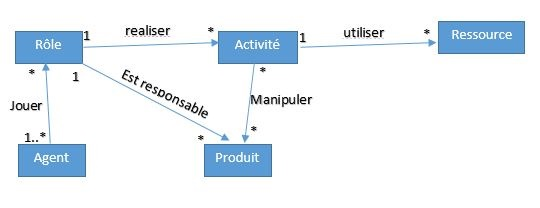
\includegraphics[width=13cm]{modeleProcede.jpg}
\caption{\label{mcp}Modèle conceptuel de procédés~\cite{hnt10}}
\end{figure}
\subsection{Langage de modélisation de procédés }
Pour décrire un modèle de procédé, nous avons besoin de langage, ce langage est appelé \og Langage de modélisation de procédés \fg{} ou \textit{"Process Modeling Language (PML)"}~\cite{ac}~\cite{rc}~\cite{sl} ou encore \textit{"Software Process Modeling Language (SPML)"}~\cite{alm}. \\
Ils existent plusieurs langages de modélisation de procédés logiciel, mais d'après les études de~\cite{abgm},\cite{vra}~\cite{jab}, les propriétés les plus importantes attendues d'un PML sont:
\begin{enumerate}
\item Formalisation: cette propriété représente le degré de formalisation (définition syntaxique) et de la sémantique du PML. Il existe trois degrés de formalisation: formel \footnote{un langage formel est un langage dont la sémantique et la syntaxe sont bien définis}, informel \footnote{langage non défini avec des concepts, une syntaxe et une sémantique}, semi-formel\footnote{langage dont la syntaxe est précise mais la sémantique non}.
\item Expressivité: cette catégorie reflète la capacité du PML à représenter tous les éléments du procédé.
\item Compréhensibilité: elle peut être textuel ou graphique, cette propriété reflète le degré de facilité à comprendre le modèle décrit à travers la notation du PML.
\item Abstraction et modularité: elles représentent la capacité du PML à proposer des mécanismes d'abstraction et d'agrégation afin de structurer les procédés pour une facilitation de la réutilisation.
\item Exécutabilité: c'est la capacité du PML à représenter des modèles exécutables (opérationnels). 
\item Évolutivité: c'est la capacité de supporter l'évolution de modèles de procédé. 
\item Multi-vue: la capacité à supporter les modèles d'activités, produits, rôles, ressources 
\end{enumerate}
En étudiant les PMLs, on s'aperçoit qu'ils peuvent utilisés différentes approches afin de mieux répondre aux besoins de la phase. Nous n'allons pas citer toutes les approches existantes, mais nous présenterons quelques une des plus connues. Parmi ces approches nous avons:
\begin{itemize}
\item approche procédurale: proposée dans~\cite{lo}, l'approche procédurale permet de représenter le modèle de procédé sous la forme d'un programme. Ce programme décrit de manière détaillé comment le procédé logiciel doit être réalisé.
\item approche déclarative: cette approche utilise des déclarations logiques (règles) pour décrire les procédés logiciels. Ceux-ci sont décrits en termes de résultats attendus par l'utilisateur sans détailler la manière dont ces résultats sont obtenus~\cite{lgw}.
\item approche fonctionnelle: l'approche fonctionnelle définit le procédé logiciel à travers un ensemble de fonctions mathématiques. Chaque fonction est décrite en termes de relations entre les données d'entrée et les données de sortie. 
\item approche basée sur les réseaux de pétri: cette approche permet de décrire le procédé logiciel à travers un réseau de pétri\footnote{un réseau de pétri est un moyen de: \\ - modélisation du comportement des systèmes dynamiques à évènements discrets;\\ - description des relations existantes entre des conditions et des évènements}.
\item approche basée sur UML: cette approche utilise des diagrammes UML pour représenter les concepts du procédé et renforce la sémantique de ces diagrammes avec un langage formel pour rendre les modèles de procédé à la fois compréhensifs et exécutables. 
Plusieurs approches ont été développées avec cette perspective, notamment le standard de l'OMG\footnote{société Américaine créée en 1989, il est à la base des standards UML, MOF \textit{"Meta-Object Facility"}, CORBA \textit{"Common Object Request Broker Architecture"}, CWM \textit{"Common Warehouse Metamodel"}} \textit{"Object Management Group"} SPEM.
\subsubsection*{\textit{Software Process Engineering Metamodel} (SPEM)}\label{spemomglabel}
le méta-modèle d'ingénierie des procédés logiciels est à la fois un méta-modèle (c'est un langage de modélisation permettant d'exprimer les concepts conforme au MOF) et un profil UML (il est basé sur du UML). Le leitmotiv d'un SPEM est qu'un procédé de développement de logiciel est une collaboration entre des entités actives et abstraites (les rôles) qui effectuent des opérations appelés activités, sur des entités concrètes qui sont les produits (Figure~\ref{mcpomg}).\\
\begin{figure}[h]
\centering
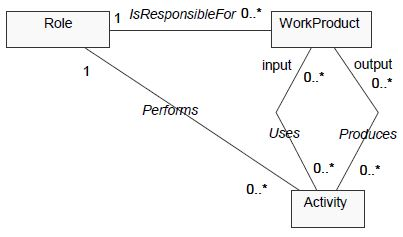
\includegraphics[width=10cm]{mcdspem.jpg}
\caption{\label{mcpomg}Modèle conceptuel de SPEM~\cite{omg1}}
\end{figure}
\clearpage
Aujourd'hui, il existe deux versions de SPEM: le \textbf{SPEM 1.1} et le \textbf{SPEM 2.0}.
\begin{itemize}
\item[\tiny{$\blacktriangleright$}] SPEM 1.1: c'est la première version de SPEM, adopté en janvier 2005, il est composé de deux groupes: le \textit{SPEM foundation} qui fournit les concepts de base pour définir le méta-model SPEM (Figure.~\ref{modele}) et le \textit{SPEM-Extension} qui décrit le concept de base pour décrire les processus logiciels. 
\begin{figure}[h] 
\centering
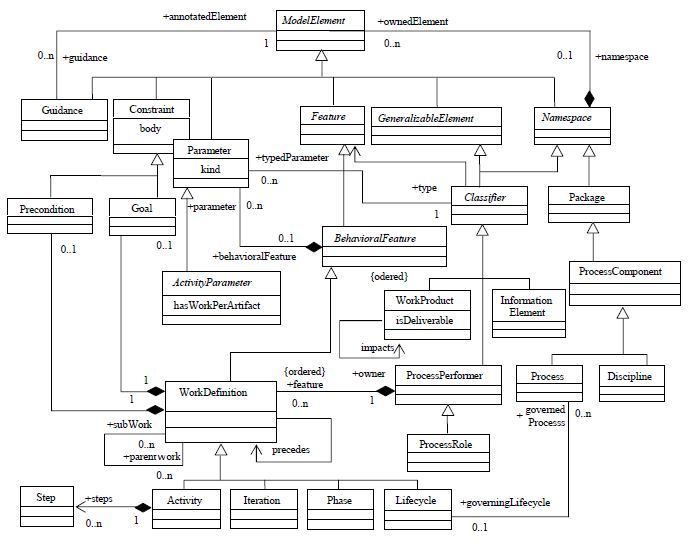
\includegraphics[width=16cm]{meta1.jpg}
\caption{\label{modele}Méta-modèle de SPEM 1.1~\cite{omg1}}
\end{figure}
\item[\tiny{$\blacktriangleright$}] SPEM 2.0: c'est la version la plus récente de SPEM depuis 2008. Comme on peut le voir sur la figure~\ref{sspem}, SPEM 2.0 est composé de sept paquetages.
\clearpage
\begin{figure}[h]
\centering
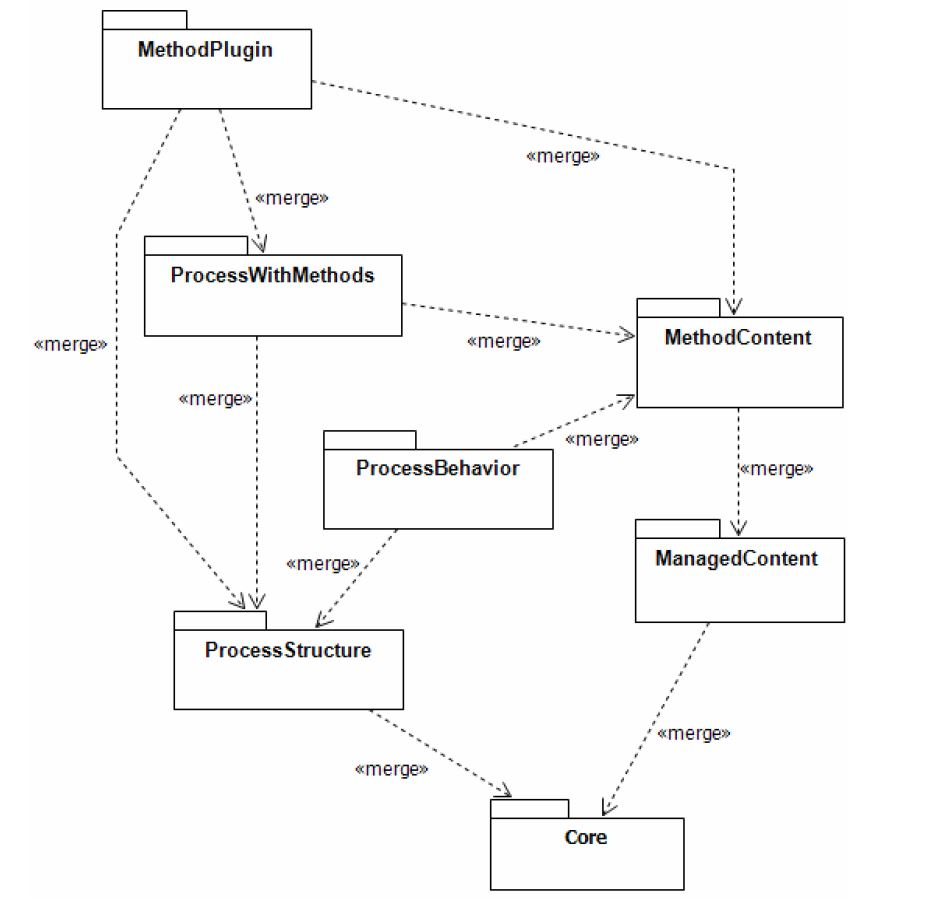
\includegraphics[width=14cm]{strucspem.jpg}
\caption{\label{sspem}Structure du SPEM 2.0~\cite{omg2}}
\end{figure}
\begin{itemize}
\item[\tiny{$\blacksquare$}] \textbf{ \textit{MethodPlugin}}: dans ce paquetage, seront gérés les librairies et les référentiels méthodologiques.
\item[\tiny{$\blacksquare$}] \textbf{ \textit{ProcessWithMethods}}: ce paquetage permet de définir ou de redéfinir les éléments pour intégrer les processus définis avec les concepts du paquetage \textit{ProcessStructure}, selon les contenus définis avec les concepts du paquetage \textit{MethodContent};
\item[\tiny{$\blacksquare$}] \textbf{ \textit{MethodContent}}: ce paquetage fournit les concepts pour que les utilisateurs puissent spécifier le contenu des méthodes comme les rôles \textit{(Roles)}, les tâches \textit{(Tasks)}, etc.; 
\item[\tiny{$\blacksquare$}] \textbf{ \textit{ProcessBehavior}}: il offre la possibilité de lier un élément de procédé SPEM 2.0 avec un comportement externe comme un modèle BPMN \textit{(Business Process Modeling Notation)} ou un modèle UML 2.
\item[\tiny{$\blacksquare$}] \textbf{ \textit{ManagedContent}}: ce paquetage fournit les concepts pour gérer les descriptions textuelles des éléments de procédés.
\item[\tiny{$\blacksquare$}] \textbf{ \textit{ProcessStructure}}: ce paquetage définit la base pour représenter tous les modèles de procédés.
\item[\tiny{$\blacksquare$}] \textbf{ \textit{Core}}: il contient les éléments de base (classes et abstractions) utilisés dans les autres paquetages. 
\end{itemize}
\end{itemize} 
\end{itemize}
Après la présentation des modèles de procédés et des langages de modélisation, nous allons passer aux environnements de génie logiciel centrés procédé.
\section{Process-Centered Software Engineering Environments (PSEE)}
Un PSEE est un environnement de travail permettant de fournir divers services aux développeurs par l'exécution des modèles de processus. Ces services sont multiples, parmi lesquels nous avons : l'aide aux développeurs logiciel, l'automatisation de certaines tâches, l'invocation et le contrôle des outils de développement logiciel, le contrôle de l'application des règles obligatoires, etc.~\cite{vra}. \\
La figure~\ref{rolepsee} résume le rôle d'un PSEE dans le processus de développement d'un logiciel.
\begin{figure}[h]
\centering
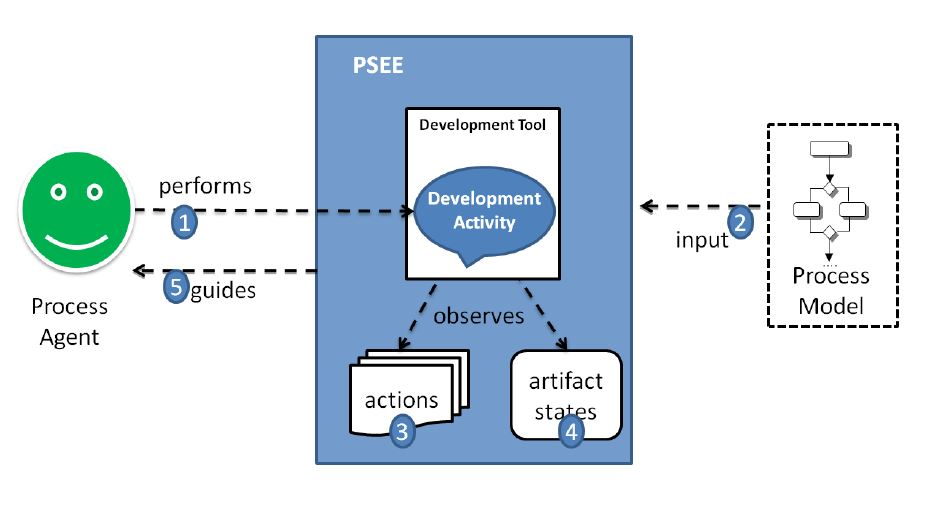
\includegraphics[width=13cm]{role.jpg}
\caption{\label{rolepsee}Rôle d'un PSEE~\cite{alm}}
\end{figure}
\clearpage
Le PSEE prend en entrée le modèle de procédé et permet à l'agent de réaliser l'activité de \og développement de logiciel \fg{}. Dans le but de s'assurer que les activités en cours respectent le modèle de processus définit, le PSEE observe les actions effectuées par les agents. Si les agents ne suivent pas les processus définis, le PSEE doit les guider dans la bonne direction. Le fait d'exécuter une action ne respectant pas les règles décrit dans le modèle de procédé est appelée \textbf{\og variation \fg{}} ou \textbf{\og déviation \fg{}}.  
Il existe plusieurs PSEE, mais la plupart ne supportent pas la notion de la gestion de variation dans le processus de développement du logiciel. Dans cette partie, nous allons faire une présentation de certains PSEE et également la manière dont ils gèrent les variations par rapport au prévisionnel.
\subsection*{EPOS}
Développé à l'université norvégienne de sciences et de technologie, EPOS est un PSEE assez complet pour la gestion des configurations et la modélisation des procédés logiciels.
Il comporte un ensemble d'outils de procédés et utilise SPELL (Software Process Evolutionary Language) comme PML.
Dans EPOS, l'élément principal est un système de base de données \og EPOSDB \fg{} dans laquelle sont stockées les objets et les instances de procédé~\cite{capri}. 
Le modèle de procédé logiciel dans EPOS est décrit comme étant un réseau de description de tâches ou d'activités lié entre elles.\\
L'architecture d'EPOS est composée de plusieurs couches~\cite{tpme} qui sont:
\begin{enumerate}
\item EPOSDB, celle ci constituant le système de base de données, offre un modèle orientée objet de donnée~\footnote{les informations sont stockées sous forme de collections d'objets persistants} pour définir les entités et la relation entre les classes. Les relations entre chaque entité avec leurs classes et méta-classes sont stockées dans la base de données.
\item Un PML réfléchi~\footnote{La réflexion est la capacité à un programme d'examiner et de contrôler son propre implémentation} et orienté objet, cette couche permet de supporter l'analyse, la conception, la personnalisation et l'évolution des méta-activités.
\item Une couche pour gérer la concurrence entre les modèles de procédés logiciel.
\item Une dernière couche pour les modèles de procédé spécifique à l'application. C'est les domaines spécifiques avec les schémas.
\end{enumerate}
A chaque tâche est associée des pré et post-conditions, les pré-conditions sont eux même divisées en deux parties: une partie statique, utilisé à l'instanciation de la tâche; et une partie dynamique qui est testée par le gestionnaire d'exécution au moment de son exécution~\cite{capri}.
EPOS est capable de détecter quelques variations liées à la structure et à l'organisation, mais il est incapable de faire une détection le plus rapidement possible et ne propose pas non plus de risque associé à la variation détectée~\cite{alm2224}.
\subsection*{RHODES}
Développé à l'ENSEEIHT-IRIT à Toulouse, RHODES est un PSEE utilisant le langage PBOOL+ comme PML; Le PBOOL+ permet de définir les composants (activités, rôles, produits et stratégies) des processus et les comportements attendus~\cite{si}. 
Comme on le voit sur la figure \ref{rhodesArch} l'architecture de RHODES est composée de deux niveaux: statique et dynamique. Le niveau statique se compose: du méta-modèle, de la base de composant de procédé, du composant d'éditeur de procédé, du noyau d'exécution et du compilateur PBOOL+. Le niveau dynamique est constitué d'une instance exécutable de procédé.
\begin{figure}[h]
\centering
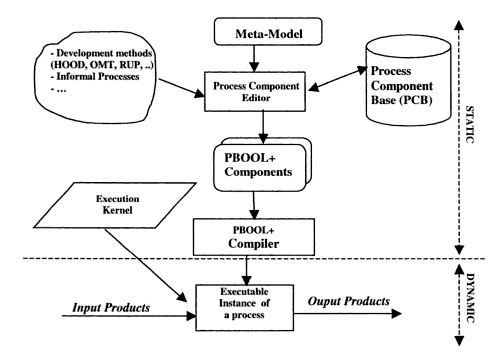
\includegraphics[width=13cm]{rhodes.jpg}
\caption{\label{rhodesArch}Architecture de RHODES~\cite{si}}
\end{figure}
Le fait de pouvoir définir comment l'activité est supposée être exécutée grâce à PBOOL+, permet à RHODES de détecter la plupart des variations car si on est capable de définir la manière d'exécution ou le comportement attendu d'une activité, il suffit après de faire une comparaison pour savoir si oui ou non nos conditions ont été respectées. En revanche il ne présente pas de mécanisme capable d'estimer ou d'évaluer le risque associé à une variation~\cite{almRhodes}.
\subsection*{SPADE}
L'acronyme de \emph{Software Process Analysis, Design and Enactment}, SPADE est un PSEE développé à Politecnico di Milano et CEFRIEL. Son PML appelé SLANG est basé sur une extension des réseaux de pétri: ER nets~\cite{link1}~\cite{link2}. L'architecture de SPADE est centrée sur le principe de séparation entre l'interprétation des modèles de procédé et l'interaction utilisateur. \\
SPADE est composé de trois couches~\cite{link1}:
\begin{enumerate}
\item l'environnement d'exécution des procédés, dans cet environnement sont exécutés nos procédés décrits avec SLANG. Les artéfacts crées ou modifiés sont stockés dans une base de données orientées objet DBMS.
\item l'environnement d'interaction avec l'utilisateur, dans cet environnement est géré tout ce qui est interaction entre l'utilisateur et les outils dans l'environnement.
\item Filtre, il est l'intermédiaire entre l'environnement d'exécution des procédés et celui d'interaction utilisateur. Son rôle est de convertir les messages générés depuis l'environnement d'interaction utilisateur, les transformer en jetons pour qu'ils puissent être exécutés dans l'environnement d'exécution. Et inversement il transforme les résultats des travaux effectués par l'interpréteur SLANG et les convertissent en message à destination de l'utilisateur.
\end{enumerate}
\begin{figure}[h]
\centering
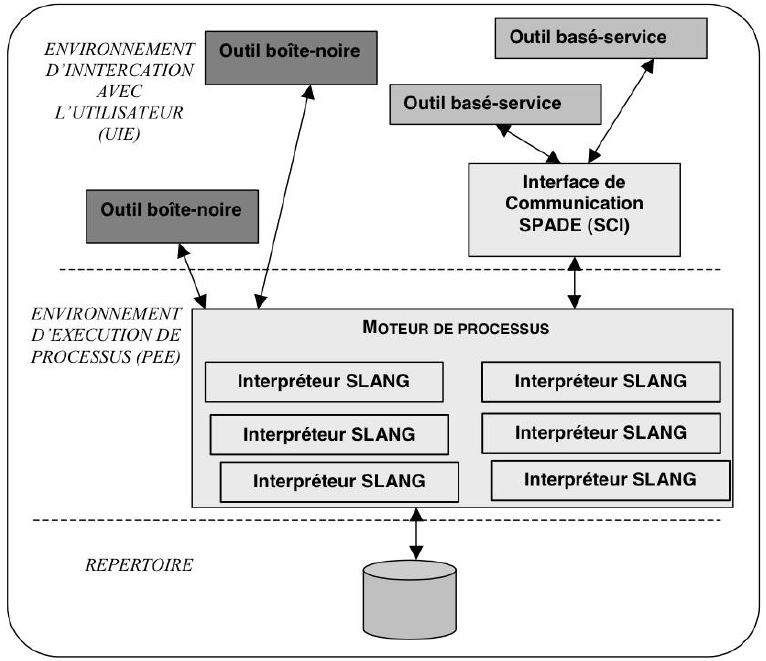
\includegraphics[width=13cm]{spade.jpg}
\caption{\label{spadeArch}Architecture de SPADE~\cite{spadeArch}}
\end{figure}

 
\chapter{Gestion des variations} % Main chapter title

\label{Chapitre3} % For referencing the chapter elsewhere, use \ref{Chapter1} 
\lhead{Chapitre 3. \emph{Gestion des variations}} % This is for the header on each page - perhaps a shortened title
Une variation est considéré comme toute action non définie dans le modèle de procédé initiale ou qui viole certaines contraintes de procédés.
Après une étude de l'existant, nous allons proposer deux solutions de gestion de variations. La première solution consiste à traiter les variations grâce à un PSEE; la seconde solution quand à elle, utilise un fichier excel pour gérer les variations.
Alors cette partie sera composée de nos techniques de détection de variations (la technique à l'aide d'un PSEE et la seconde technique à l'aide d'un fichier excel).
\section{Solution 1}
Comme nous l'avons dit dans le chapitre~\ref{Chapitre2}, l'OMG a proposé en 2005 le SPEM 1.1, mais ce dernier présentant quelques lacunes, ils ont proposé en 2008 une nouvelle version (SPEM 2.2). 
Ces normes de l'OMG sont utilisés dans de nombreux travaux de recherches car ils sont considérés aujourd'hui comme étant un modèle assez complet pour pouvoir décrire les procédés. Alors pour cette première solution, je me suis beaucoup basé sur les solutions proposées par l'OMG dans leurs travaux.
\subsection{Méta-modèle de procédé}
Avant d'expliquer la technique de détection, nous allons définir notre méta-modèle de procédé c'est à dire notre modèle définissant les concepts de base d'un langage de description de procédés.
La figure~\ref{metamodele} représente notre méta-modèle de procédé. Nous avons récupéré les éléments importants proposés par l'OMG et avons rajouter nos éléments pour nous permettre de détecter et de corriger les variations.

\begin{figure}[h]
\centering
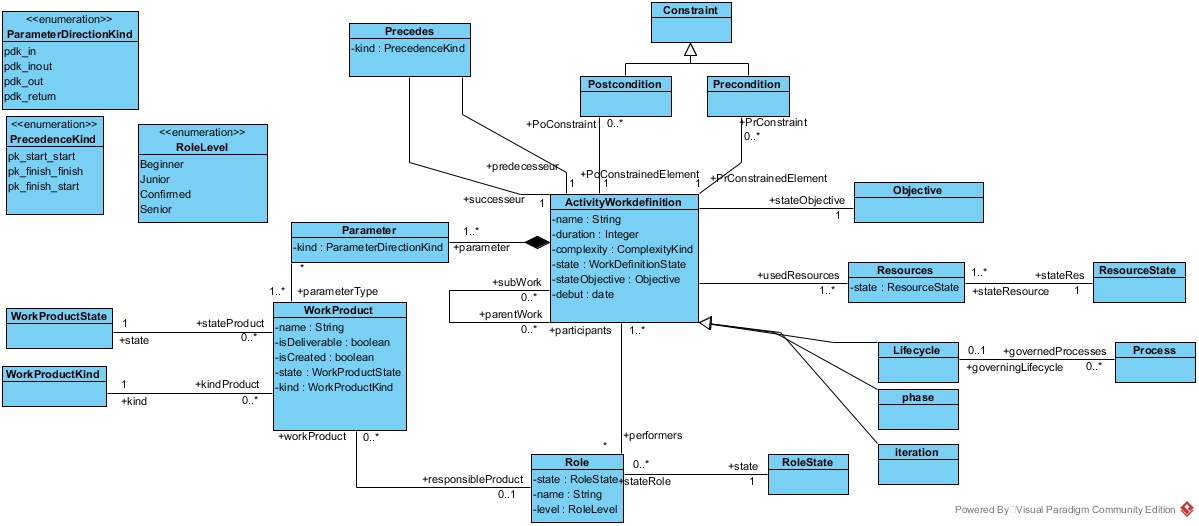
\includegraphics[width=16cm]{Solution.jpg}
\caption{\label{metamodele}Méta-modèle de SPEM solution}
\end{figure}

Nous allons maintenant décrire chaque élément de notre méta-modèle.
\subsubsection*{ActivityWorkDefinition}
L'élément \textbf{\textit{ActivityWorkDefinition}} représente un travail ou une tâche à réaliser durant le processus de développement logiciel. Ces tâches doivent être réalisées par des acteurs décrits par \textit{Role} pendant une durée donnée.\\
Les attributs de cet élément sont:\\
\begin{itemize}
\item[\tiny{$\blacksquare$}] Name: c'est une chaine de caractère qui correspond au nom de la tâche.
\item[\tiny{$\blacksquare$}] State: de type \textit{ActivityWorkDefinitionState}, il permet de connaitre l'état de la tâche.
\item[\tiny{$\blacksquare$}] Duration: nombre représentant la durée de la tâche.
\item[\tiny{$\blacksquare$}] Complexity: indique le niveau de difficulté ou le degré de complexité de la tâche. Il pourra nous être utile pendant le traitement d'une déviation.
\item[\tiny{$\blacksquare$}] stateObjective: attribut de type \textit{Objective}, il indique l'objectif ou le but du travail.
\end{itemize}
\subsubsection*{WorkProduct, WorkProductKind, WorkProductState}
L'élément \textbf{\textit{WorkProduct}} ou artéfact représente tout ce qui est produit, modifié ou consommé par un \textit{ActivityWorkDefinition}. Ses attributs sont:\\
\begin{itemize}
\item[\tiny{$\blacksquare$}] Name: chaine de caractère représentant le nom du produit.
\item[\tiny{$\blacksquare$}] isDeliverable: booléen permettant de savoir si le produit peut être délivré ou pas.
\item[\tiny{$\blacksquare$}] Kind: de type \textit{WorkProductKind}, il permet de connaitre le type du produit c'est à dire si c'est un document, model ou code.
\item[\tiny{$\blacksquare$}] State: indique l'état du produit, il est de type \textit{WorkProductState}.
\item[\tiny{$\blacksquare$}] isCreated: booléen permettant de savoir si le produit fut crée ou pas par la tâche.
\end{itemize}
Un \textbf{\textit{WorkProductKind}} représente les catégories de produits que l'on peut avoir. Ces catégories peuvent être du code, des documents, du model etc.\\
L'élément \textit{WorkProductState} indique les états d'un produit (initial, validé, invalidé etc...)

\subsubsection*{RoleLevel, Role}
\textit{RoleLevel} est une énumération des niveaux qu'un rôle peut avoir (débutant, junior, confirmé, senior).\\
Un \textit{Role} représente les rôles ou acteurs responsables d'un produit ou contribuant à la réalisation d'une tâche. Par exemple on peut avoir des analystes, des testeurs etc... Cet élément rôle possède un attribut \textit{name} qui indique le nom du rôle;  un attribut \textit{state} indiquant l'état du rôle c'est à dire si le rôle a terminé d'accomplir la tâche ou si il est en train de le faire etc... et un attribut \textit{level} qui indique le niveau de l'acteur (débutant, junior, confirmé). 
\subsubsection*{Postcondition et Precondition}
Les éléments \textbf{\textit{Precondition}} et \textbf{\textit{Postcondition}} sont des spécialisation de la classe \textit{Constraint}. Il représentent respectivement les conditions qui doivent être satisfaites avant et après l'exécution de chaque \textit{ActivityWorkDefinition}. 
\subsubsection*{Parameter}
L'élément \textbf{\textit{Parameter}} est composé d'un attribut \textit{kind} de type \textbf{\textit{ParameterDirectionKind}} qui est une énumération des types de relations qui relie une tâche à un produit. C'est à dire qu'il permet d'indiquer si un \textit{WorkProduct} est utilisé par une \textit{ActivityWorkDefinition} tant que \og entrée \fg{}, \og sortie \fg{} ou \og entrée/sortie \fg{}. 
\subsubsection*{Precedes et PrecedenceKind}
Pour expliquer les relations qui lient nos \textit{ActivityWorkDefinition}, nous allons prendre deux tâches t1 et t2, t2 étant le successeur de t1.
L'élément \textbf{\textit{PrecedenceKind}} est une énumération des relations qui peuvent exister entre nos \textit{ActivityWorkDefinition}: 
\textit{pk\_start\_start}: ce type de relation permet d'indiquer que t2 ne pourra commencer que si t1 commence.\\
\textit{pk\_finish\_finish}: ce type de relation permet d'indiquer que t2 ne pourra terminer que si t1 l'est.\\
\textit{pk\_finish\_start}: indique que t2 ne pourra commencer qu'à la fin de t1.\\
L'élément \textbf{\textit{Precedes}} comporte un attribut \textit{kind} de type \textit{PrecedenceKind}, il indique le type d'ordonnancement qui relie les \textit{ActivityWorkDefinition}. Par exemple supposons que nos deux tâches t1 et t2 sont reliées par une liaison de type pk\_start\_start, t2 ne peut pas commencer tant que t1 n'a pas commencé.
\subsubsection*{Objective}
L'élément \textbf{\textit{Objective}} représente l'objectif ou le but de la réalisation d'une tâche. Si une tâche est terminée, on pourra vérifier si l'objectif a été atteint.
\subsubsection*{ResourceState, Resources}
\textit{ResourceState} représente les états de disponibilités des ressources.
L'élément \textbf{\textit{Ressources}} représente les différentes ressources. Ces ressources sont utilisées par des tâches selon leurs disponibilités.
\subsubsection*{LifeCycle, Phase, Iteration}
L'élément \textbf{\textit{LifeCycle}} représente le cycle de vie de logiciel par exemple\og le modèle cascade \fg{} ou\og le modèle en V\fg{}
La \textbf{\textit{Phase}} est une spécialisation de \textit{ActivityWorkDefinition}. C'est une tâche correspondant à une phase d'un cycle de vie de logiciel 
L'élément \textbf{\textit{Iteration}} est une \textit{ActivityWorkDefinition} avec des préconditions et objectif bien défini appelé \og minor milestone \fg{}.
%\subsection{Well-formedness rules}
%Nous allons donner ci-dessous la traduction en OCL de nos éléments décrits ci-dessus.
\subsection{Technique de détection des variations et guide de correction}
Cette partie explique la technique de détection des variations et les solutions pour les résoudre.
%\begin{itemize}
%\item[\tiny{$\blacksquare$}]\textbf{ActivityWorkDefinition}
%\item[\tiny{$\blacksquare$}]\textbf{WorkProduct}
%\item[\tiny{$\blacksquare$}]\textbf{Postcondition}
%\item[\tiny{$\blacksquare$}]\textbf{Precondition}
%\item[\tiny{$\blacksquare$}]\textbf{Parameter}
%\item[\tiny{$\blacksquare$}]\textbf{Precedes}
%\item[\tiny{$\blacksquare$}]\textbf{Objective}
%\item[\tiny{$\blacksquare$}]\textbf{ResourceState}
%\item[\tiny{$\blacksquare$}]\textbf{Resources}
%\item[\tiny{$\blacksquare$}]\textbf{LifeCycle}
%\item[\tiny{$\blacksquare$}]\textbf{Phase}
%\item[\tiny{$\blacksquare$}]\textbf{Iteration}
%\item[\tiny{$\blacksquare$}]\textbf{RoleState}
%\item[\tiny{$\blacksquare$}]\textbf{Role}
%\item[\tiny{$\blacksquare$}]\textbf{Process}
%\end{itemize}
\subsubsection*{Technique de détection}
Rappelons nous qu'une variation est toute actions qui violent les contraintes définis dans notre procédé.
Alors, notre technique de détection des variations est simple, elle se base sur certains attributs de notre modèle.
Ces attributs sont tous les attributs représentant des contraintes. On surveille l'exécution des procédés, avant chaque exécution, on vérifie si les conditions requises pour commencer la tâche sont satisfaites c'est à dire si la pré-condition est satisfaite, si les relations de précédence sont également satisfaite. A la fin de chaque exécution, on vérifie si les post-conditions sont remplis, si la tâche est correctement terminée et l'objectif du travail est atteint. Si on voit qu'il y'a une anomalie au niveau de la satisfaction de nos contraintes alors on signale une déviation et on propose un plan de correction au chef de projet.
\subsubsection*{Guide de correction}
Notre technique de correction est basé sur la ré-exécution de la tâche ou peut-être l'ignorer. Si une déviation est détectée, on regarde les causes ensuite on propose au chef de projet les solutions suivantes:\\
\begin{itemize}
\item[\tiny{$\blacksquare$}] ignorer la déviation si elle est mineure comme par exemple, on veut lancer une tâche dont toutes les pré-conditions sont satisfaites mais la date supposé être la date de lancement de la tâche n'est pas arrivé, alors on peut proposer au chef de projet de modifier la date ou de l'ignorer. Car ça ne va pas générer des erreurs négatives (comme un retard dans la livraison).
\item[\tiny{$\blacksquare$}] la seconde solution à analysé les causes:\\
si c'est un dépassement de la date limite du travail, on pourra proposer au chef de projet d'affecter la tâche à un rôle plus compétent si le rôle responsable de la tâche n'est pas assez compétent sinon on modifie la date limite et on laisse le même rôle continuer à exécuter la tâche. Sinon si c'est l'exécution d'une action non défini dans le modèle de procédé initial, on demande au chef de projet de redéfinir le modèle de procédé.
\end{itemize}
\section{Deuxième solution}
Pour cette deuxième solution, je me suis rapproché d'un chef de projet chez \og Alstom \fg{} afin de mettre en place cette solution. C'est une solution plus simple car elle est réalisée à l'aide d'un fichier excel.

\chapter{Conclusion} % Main chapter title

\label{Chapitre4} % For referencing the chapter elsewhere, use \ref{Chapter1} 

\lhead{Chapitre 4. \emph{Conclusion}} % This is for the header on each page - perhaps a shortened title
Dans ce travail de recherche, nous avons étudier les variations par rapport aux prévisions dans la gestion des projets informatiques. Nous avions pour objectif d'étudier les variations et de proposer un modèle de gestion de ces variations pendant la gestion du projet.\\
Nous avons proposer deux solutions: une première solution basée sur les PSEE et une seconde solution avec un fichier excel.\\
La première solution est composée de trois parties: le méta-modèle pour décrire les procédés, la technique de détection des variations et le plan de correction pour la variation détectée.\\
La seconde solution a été mise en place suite à une discussion avec un chef de projet chez Alstom. C'est un macro excel permettant de détecter les variations grâce aux paramètres qu'on lui fournit et nous affiche les résultats sous forme de graphe. \\
Même si ces solutions permettent de détecter quelques variations, et aident le chef de projet dans la prise de décision; elles ne peuvent pas détecter tous les types de variations.\\
\textbf{Limites et perspectives}: les limites et les perspectives d'amélioration de nos deux solutions sont:\\
\textbf{Solution 1}:\\
Notre première solution est assez limité car elle ne permet pas d'anticiper la détection des variations. La variation n'est détectée que lorsque les tâches sont terminées.\\
\textbf{Solution 2}:\\
Les diagrammes résultant de l'exploitation de notre modèle de fichier Excel initialement mis en place et nous permettent à travers des représentations graphiques de voir systématiquement la variation sur les dates de début et de réalisation des tâches. \\
Par rapport aux diagrammes~\ref{graphe1} et~\ref{graphe2} on pourra améliorer ces derniers en traçant une droite horizontale qui représente la date de validité (date à laquelle les données ont été mises à jour), on aurait pu séparer les taches précédentes des tâches futures à venir~\ref{graphe4}.
\begin{figure}[h]
\centering
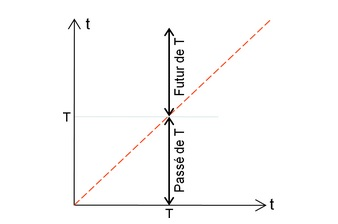
\includegraphics[width=9cm]{graphe4.jpg}
\caption{\label{graphe2}Amélioration}
\end{figure}
D'autres types d'indicateurs peuvent également être mis en  place en fonction des besoins. On pourra par exemple mettre en place un tableau de synthèse de variations qui pourra être importé dans un autre outil etc.
 
%\chapter{Conclusion} % Main chapter title

\label{Chapitre4} % For referencing the chapter elsewhere, use \ref{Chapter1} 

\lhead{Chapitre 4. \emph{Conclusion}} % This is for the header on each page - perhaps a shortened title
Dans ce travail de recherche, nous avons étudier les variations par rapport aux prévisions dans la gestion des projets informatiques. Nous avions pour objectif d'étudier les variations et de proposer un modèle de gestion de ces variations pendant la gestion du projet.\\
Nous avons proposer deux solutions: une première solution basée sur les PSEE et une seconde solution avec un fichier excel.\\
La première solution est composée de trois parties: le méta-modèle pour décrire les procédés, la technique de détection des variations et le plan de correction pour la variation détectée.\\
La seconde solution a été mise en place suite à une discussion avec un chef de projet chez Alstom. C'est un macro excel permettant de détecter les variations grâce aux paramètres qu'on lui fournit et nous affiche les résultats sous forme de graphe. \\
Même si ces solutions permettent de détecter quelques variations, et aident le chef de projet dans la prise de décision; elles ne peuvent pas détecter tous les types de variations.\\
\textbf{Limites et perspectives}: les limites et les perspectives d'amélioration de nos deux solutions sont:\\
\textbf{Solution 1}:\\
Notre première solution est assez limité car elle ne permet pas d'anticiper la détection des variations. La variation n'est détectée que lorsque les tâches sont terminées.\\
\textbf{Solution 2}:\\
Les diagrammes résultant de l'exploitation de notre modèle de fichier Excel initialement mis en place et nous permettent à travers des représentations graphiques de voir systématiquement la variation sur les dates de début et de réalisation des tâches. \\
Par rapport aux diagrammes~\ref{graphe1} et~\ref{graphe2} on pourra améliorer ces derniers en traçant une droite horizontale qui représente la date de validité (date à laquelle les données ont été mises à jour), on aurait pu séparer les taches précédentes des tâches futures à venir~\ref{graphe4}.
\begin{figure}[h]
\centering
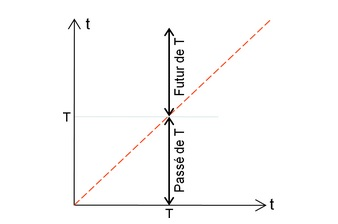
\includegraphics[width=9cm]{graphe4.jpg}
\caption{\label{graphe2}Amélioration}
\end{figure}
D'autres types d'indicateurs peuvent également être mis en  place en fonction des besoins. On pourra par exemple mettre en place un tableau de synthèse de variations qui pourra être importé dans un autre outil etc.
 
%\input{Chapters/Chapter6} 
%\input{Chapters/Chapter7} 


%----------------------------------------------------------------------------------------
%	BIBLIOGRAPHY
%----------------------------------------------------------------------------------------

\label{Bibliographie}

\lhead{\emph{Bibliographie}} % Change the page header to say "Bibliography"

\bibliographystyle{unsrtnat} % Use the "unsrtnat" BibTeX style for formatting the Bibliography

\bibliography{Bibliography} % The references (bibliography) information are stored in the file named "Bibliography.bib"

\end{document}  